\begin{greek}
\chapter{Γενεαλογική συλλογή σκουπιδιών}\label{ch:gen}

Ο στόχος ενός συλλέκτη σκουπιδιών είναι η εύρεση νεκρών αντικειμένων
και εν συνεχεία η αποδέσμευση του χώρου που αυτά καταλαμβάνουν.
Οι συλλέκτες εξιχνίασης (και ειδικότερα οι συλλέκτες με αντιγραφή)
παρουσιάζουν καλές επιδόσεις όταν ο σωρός περιλαμβάνει σχετικά
λίγα ζωντανά αντικείμενα. Δε μεταχειρίζονται ωστόσο αποδοτικά
αντικείμενα με μακρά διάρκεια ζωής, τα οποία είτε σημαίνουν και
ξε-σημαίνουν είτε αντιγράφουν από τον ένα ημιχώρο στον άλλο
διαρκώς. Είδαμε στο κεφάλαιο~\ref{ch:mrkcmp} πώς αντικείμενα με
μακρά διάρκεια ζωής τείνουν να συγκεντρώνονται στο κάτω μέρος
του σωρού όταν αυτός διαχειρίζεται από ένα συλλέκτη με σήμανση
και συμπύκνωση και πώς πολλοί συλλέκτες αποφεύγουν τη συμπύκνωση
αυτού του τμήματος. Παρότι αυτή η βελτιστοποίηση αφαιρεί το κόστος
της μετακίνησης αυτών, τα εν λόγω αντικείμενα πρέπει να εξετάζονται
και τα πεδία δείκτες αυτών να ενημερώνονται σε κάθε κύκλο συλλογής. 

Οι γενεαλογικοί συλλέκτες σκουπιδιών επεκτείνουν την παραπάνω
ιδέα αγνοώντας τα παλαιότερα αντικείμενα οποτεδήποτε αυτό είναι
δυνατό. Οι συλλέκτες αυτής της κατηγορίας βασίζονται στην ασθενή
γενεαλογική υπόθεση πώς τα περισσότερα αντικείμενα πεθαίνουν νέα.
Επικεντρώνοντας την προσοχή τους στα νεότερα αντικείμενα, προσπαθούν
να μεγιστοποιήσουν τον ελεύθερο χώρο που ανακτούν με το λιγότερο
δυνατό κόπο. Κατηγοριοποιούν τα αντικείμενα με βάση την ηλικία
τους σε γενεές, με την κάθε γενιά να ζει συνήθως σε ένα ξεχωριστό
τμήμα του σωρού. Οι γενεές συλλέγονται σε αύξουσα σειρά ως προς
την ηλικία  τους, ενώ  τα αντικείμενα που επιβιώνουν μετά από
αρκετούς κύκλους συλλογής προάγονται σε παλαιότερες γενεές.

Οι περισσότεροι συλλέκτες αυτής της κατηγορίας διαχειρίζονται
τις νεότερες γενεές με αντιγραφή. Ο απαιτούμενος χρόνος που
δαπανάται για τη νεότερη γενεά, γνωστή και ως βρεφοκομείο εξαρτάται
από το μέγεθός της. Ρυθμίζοντας επομένως το μέγεθος αυτό, μπορούμε
να ελέγξουμε το χρόνο παύσης για τη συλλογή μιας γενεάς. Οι χρόνοι
παύσης για τη συλλογή των νεότερων γενεών σε εφαρμογές που τρέχουν
σε ένα σύγχρονο μηχάνημα και οι οποίες επαληθεύουν την ασθενή
γενεαλογική υπόθεση είναι της τάξης των χιλιοστών του δευτερολέπτου.
Θεωρώντας ακόμη πώς η συλλογή εκτελείται σχετικά αραιά, η δράση
ενός γενεαλογικού συλλέκτη περνάει σχεδόν απαρατήρητη στον τροποποιητή.

Αν ένας γενεαλογικός συλλέκτης εκτιμήσει πώς η συλλογή μόνο
της νεότερης γενιάς δε θα ανακυκλώσει αρκετό χώρο, χρειάζεται
να συλλεχθεί ολόκληρος ο σωρός. Συνεπώς η γενεαλογική συλλογή
σκουπιδιών βελτιώνει μόνο την αναμενόμενη τιμή του χρόνου παύσης
και όχι την χείριστη περίπτωση. Δεν επαρκεί από μόνη της για ένα
σύστημα πραγματικού χρόνου.

Η \textbf{γενεαλογική συλλογή σκουπιδιών} δεν είναι τελείως
δωρεάν. Αρχικά η συνεχόμενη συλλογή μόνο των νεότερων γενεών
δεν μπορεί να εντοπίσει σκουπίδια που ζουν σε παλαιότερες γενεές.
Επιπλέον, για να μπορεί να συλλέξει μόνο μια γενεά, αγνοώντας
τις υπόλοιπες, ο συλλέκτης θα πρέπει με κάποιο τρόπο να σημειώνει
τους δείκτες που διασχίζουν τα σύνορα μεταξύ των γενεών.

\section{Πώς μετράται ο χρόνος;}
Για να πρoάγει ένας γενεαλογικός συλλέκτης αντικείμενα από μία γενεά σε μία 
παλαιότερη, απαιτείται να μπορεί να προσδιορίζει πόσο παλαιά αυτά είναι. 
Επομένως χρειάζεται τόσο ένα μηχανισμό μέτρησης του χρόνου όσο και ένα μηχανισμό 
μέτρησης της ηλικίας των αντικειμένων. Στη βιβλιογραφία συναντώνται κυρίως δύο 
πιθανές μετρικές: το συνολικό μέγεθος της δεσμευμένης μνήμης και ο χρόνος που 
έχει περάσει από την έναρξη της εκτέλεσης της εφαρμογής. Η μετρική του χρόνου 
καθορίζει το προφίλ της εφαρμογής. Απαντάει σε ερωτήσεις που αφορούν το για πόσο 
τρέχει μια εφαρμογή καθώς και ποιοι είναι οι χρόνοι παύσης αυτής και είναι 
κατανεμημένοι. Απαντήσεις στις ερωτήσεις αυτές μπορούν να χρησιμοποιηθούν ώστε 
να αποφανθεί κανείς σχετικά με την αποκρισιμότητα της εφαρμογής και το κατά πόσο 
η διακοπή αυτής για συλλογή σκουπιδιών ενοχλεί έναν διαδραστικό χρήστη. Από την 
άλλη πλευρά, εσωτερικά, η διαφορά σε bytes της συνολικής δεσμευμένης μνήμης στο 
σωρό μεταξύ των χρονικών στιγμών της γέννησης και του θανάτου ενός αντικειμένου 
αντικατοπτρίζει καλύτερα τη χρονική διάρκεια ζωής αυτού. Είναι επίσης ένα μέγεθος 
ανεξάρτητο της αρχιτεκτονικής. Τέλος, αποτελεί στοιχείο των απαιτήσεων σε μνήμη 
μιας εφαρμογής και είναι στενά συνδεδεμένο με τη συχνότητα με την οποία θα κληθεί 
ο συλλέκτης. Η μέτρηση του χρόνου με όρους bytes είναι ιδιαίτερα επίπονη διαδικασία 
σε πολυεπεξεργαστικά περιβάλλοντα όπου εκτελούνται ταυτόχρονα πολλά νήματα. Η χρήση 
ενός απλού καθολικού μετρητή του συνολικού μεγέθους της δεσμευμένης μνήμης ενδέχεται 
να παραπλανήσει το συλλέκτη σχετικά με την ηλικία ενός αντικειμένου, καθώς μια 
μεγάλη τιμή του μπορεί να έχει προκύψει από την εκχώρηση μνήμης σε νήματα άσχετα 
με το αντικείμενο. Οι πραγματικές υλοποιήσεις γενεαλογικών συλλεκτών σκουπιδιών 
μοντελοποιούν την ηλικία ενός αντικειμένου ως τον αριθμό των συλλογών από τις 
οποίες αυτό έχει επιβιώσει.

\section{Γενεαλογικές υποθέσεις}
\textbf{H ασθενής γενεαλογική υπόθεση}, σύμφωνα με την οποία
τα περισσότερα αντικείμενα πεθαίνουν νέα, φαίνεται γενικώς
έγκυρη, ανεξαρτήτως της γλώσσας προγραμματισμού. Οι Foderaro
και Fateman \cite{DBLP:conf/issac/FoderaroF81} διαπίστωσαν
πώς σε ένα πακέτο υπολογιστικής άλγεβρας γραμμένο στη γλώσσα
MacLisp, το 98\% της μνήμης που ανακτούσε ένας κύκλος συλλογής
είχε εκχωρηθεί μετά το πέρας του προηγούμενου κύκλου. Ο Zorn
\cite{Zorn:CSD-89-544} ανέφερε πώς το ποσοστό των αντικειμένων
στη γλώσσα Common Lisp τα οποία επιβίωναν λιγότερο από 10 ΚΒ
εκχώρησης κυμαίνεται μεταξύ 50\% και 90\%. Αντίστοιχα συμπεράσματα 
ισχύουν και για τις συναρτησιακές γλώσσες προγραμματισμού. Οι
Sansom και Simon Peyton Jones \cite{DBLP:conf/fpca/SansomJ93},
παρατήρησαν, πώς στη Haskell, ένα ποσοστό μεταξύ 75\% και 95\%
των αντικειμένων του σωρού πεθαίνουν πριν την ηλικία των 10 KB
και πώς μόνο το 5\% των αντικειμένων ζουν περισσότερο από 1 ΜΒ.
Ο Appel παρατήρησε πώς στην Standard ML/NJ, σε κάθε κύκλο
συλλογής, το 98\% της μνήμης κάθε γενεάς ελευθερώνεται, ενώ
οι Stefanovic και Moss \cite{DBLP:conf/lfp/StefanovicM94}
βρήκαν πώς μόνο ένα ποσοστό από 2\% έως 8\% αντικειμένων του
σωρού επιβίωναν μετά το κατώφλι των 100 ΚΒ.

Η υπόθεση ισχύει και για πολλά προγράμματα γραμμένα σε
αντικειμενοστρεφείς γλώσσες. Ο Ungar \cite{Ungar:CSD-86-287}
βρήκε πώς λιγότερο από το 7\% των αντικειμένων στη Smalltalk
ζουν πέραν των 140 KB. Οι Dieckmann και H{\"o}lzle
\cite{DBLP:conf/ecoop/DieckmannH99} ανέφεραν πώς ο όγκος των
ζωντανών Java αντικειμένων στη σουίτα benchmark SPECjvm98
που επιβίωναν τα 100 KB εκχώρησης κυμαινόταν μεταξύ 1\%
και 40\% και πώς λιγότερο από το 21 \% ζούσε πέραν του 1 ΜΒ
παρότι το ποσοστό διέφερε σημαντικά από εφαρμογή σε εφαρμογή.
Ο Blackburn κ.ά \cite{DBLP:conf/oopsla/BlackburnGHKMBDFFGHHJLMPSVDW06}
βρήκαν πώς κατά μέσο όρο ένα ποσοστό μικρότερο του 9\% των
αντικειμένων που εκχωρούνταν στις εφαρμογές των σουιτών
benchmark SPECjvm98 και DaCapo γλίτωνε από τα 4 MB παρότι
υπήρχε μεγάλη απόκλιση ανάμεσα στα διαφορετικά benchmark.
Αυτό βέβαια ήταν ένα άνω φράγμα του ποσοστού των αντικειμένων
που ζούσαν πέραν των 4 MB, καθώς μερικά επιζώντα αντικείμενα
μπορεί να γλίτωναν καθώς εκχωρούνταν σχεδόν αμέσως μετά από
μια συλλογή της νεότερης γενεάς. Οι Jones και Ryder \cite{DBLP:conf/iwmm/JonesR08}
πώς η διάρκεια ζωής των αντικειμένων εφαρμογών Java ακολουθούσαν
τη διωνυμική κατανομή: ένα ποσοστό μεταξύ 65\% και 96\% των
αντικειμένων στις εφαρμογές της σουίτας benchmark DaCapo
δεν επιβίωναν μετά τα 64 KB, ενώ ένα ποσοστό μεταξύ 3\%
και 16\% ήταν αθάνατα ή ζούσαν και πέραν των 4 MB. Ακόμη
και στις προστακτικές γλώσσες προγραμματισμού όπου δεν υπάρχει
αυτόματη διαχείριση μνήμης, η διάρκεια ζωής πολλών αντικειμένων
είναι μικρή. Οι Barrett και Zorn \cite{DBLP:conf/pldi/BarrettZ93}
ανέφεραν πώς παραπάνω από το 50\% των εκχωρηθέντων στο σωρό
αντικειμένων πέθαιναν κάποια στιγμή πριν τα 10 KB και λιγότερο
από το 10\% επιβίωνε πέραν των 32 KB.

Από την άλλη πλευρά, υπάρχουν εμφανώς λιγότερες ενδείξεις
που να επιβεβαιώνουν την \textbf{ισχυρή γενεαλογική υπόθεση}
του Hayes \cite{DBLP:conf/oopsla/Hayes91}, σύμφωνα με την
οποία ακόμη και για τα αντικείμενα που δε δημιουργήθηκαν
πρόσφατα, ισχύει πώς τα νεότερα αντικείμενα θα έχουν μικρότερο
ρυθμό επιβίωσης από τα παλαιότερα. Το απλό μοντέλο της ασθενούς
γενεαλογικούς υπόθεσης περιγράφει ικανοποιητικά τη γενική
συμπεριφορά των αντικειμένων. Ωστόσο, εξαιρώντας τα αντικείμενα
που πεθαίνουν νέα, η δημογραφία των αντικειμένων σε μία
ευρύτερη χρονική κλίμακα είναι πιο πολύπλοκη. Οι χρόνοι
ζωής των αντικειμένων δεν είναι τυχαίοι. Όπως παρατηρούν
οι Dieckmann και H{\"o}lzle \cite{DBLP:conf/ecoop/DieckmannH99}
και οι Jones και Ryder \cite{DBLP:conf/iwmm/JonesR08}, επειδή
τα προγράμματα λειτουργούν σε φάσεις, τα αντικείμενα έχουν
την τάση να ζουν σε συστάδες και να πεθαίνουν όλα μαζί
ταυτόχρονα. Επιπλέον, ένας σημαντικό πλήθος αντικειμένων μπορεί
να μην πεθάνει ποτέ. Κάποιοι ερευνητές έχουν ακόμη ισχυρισθεί
πώς ενδέχεται να υπάρχει ένας συσχετισμός μεταξύ της διάρκειας
ζωής των αντικειμένων και του μεγέθους τους. Οι απόψεις πάντως
\cite{DBLP:conf/oopsla/CaudillW86, DBLP:conf/oopsla/UngarJ88,
DBLP:conf/pldi/BarrettZ93} σχετικά το κατά πόσο ο ισχυρισμός
είναι αληθής διαφέρουν.

\section{Γενεές και οργάνωση σωρού}
Μια ευρεία γκάμα στρατηγικών έχει προταθεί στη βιβλιογραφία για την οργάνωση των
γενεών. Οι γενεαλογικοί συλλέκτες μπορεί να χρησιμοποιούν δύο ή και περισσότερες
γενεές, οι οποίες μπορεί να διαχωρίζονται φυσικά ή λογικά. Το μέγεθος μιας γενεάς
μπορεί να είναι σταθερό και φραγμένο ή μπορεί να απαιτείται συμβιβασμός μεταξύ των 
μεγεθών των διαφόρων υποχώρων του σωρού. Μια γενεά μπορεί να είναι επίπεδη στο
εσωτερικό της ή να περιλαμβάνει έναν αριθμό από υποχώρους που χαρακτηρίζονται
με βάση την ηλικία και είναι γνωστοί ως \textbf{κάδοι (buckets)}. Μια γενεά ενδέχεται
επίσης να περιέχει το δικό της υποχώρο για μεγάλα αντικείμενα. Τέλος, κάθε γενεά
μπορεί να μεταχειρίζεται από διαφορετικό αλγόριθμο.

Οι πρωταρχικοί στόχοι της γενεαλογικής συλλογής σκουπιδιών είναι η μείωση των
χρόνων παύσης και η βελτίωση της διεκπεραιωτικής ικανότητας. Υποθέτοντας πώς η
διαχείριση της νεότερης γενεάς έχει ανατεθεί σε ένα συλλέκτη αντιγραφής, οι αναμενόμενοι
χρόνοι παύσης εξαρτώνται κατά κύριο λόγο από τον όγκο των ζωντανών αντικειμένων
που επιβιώνουν από μία \textbf{μικρή (minor)} συλλογή της γενεάς αυτής, ο οποίος
με τη σειρά του εξαρτάται από το μέγεθος αυτής. Αν ωστόσο το μέγεθος του βρεφοκομείου
είναι πολύ μικρό και συνεπώς η συλλογή πολύ γρήγορη, το ποσό της μνήμης που θα 
ελευθερωθεί θα είναι μικρό, καθώς τα αντικείμενα του βρεφοκομείου δεν έχουν
επαρκή χρόνο για να πεθάνουν. Το γεγονός αυτό ενδέχεται να έχει πολλές ανεπιθύμητες
επιπτώσεις. 

Πρώτον, θα αυξηθεί σημαντικά η συχνότητα συλλογής της νεότερης γενεάς. Παράλληλα, το 
κόστος της αντιγραφής, το οποίο είναι ανάλογο του πλήθους των αντικειμένων που επιβιώνουν 
αναμένεται να αυξηθεί επίσης, δεδομένου ότι τα αντικείμενα θα έχουν λιγότερο χρόνο
ώστε να πεθάνουν. Επίσης, κάθε κύκλος συλλογής απαιτεί την αναστολή των νημάτων του
τροποποιητή και το σκανάρισμα της στοίβας κάθε νήματος.

Δεύτερον, η παλαιότερη γενεά αναμένεται να γεμίσει πολύ γρήγορα με συνέπεια να χρειαστεί
να συλλεγεί και αυτή συντομότερα. Υψηλοί ρυθμοί προώθησης θα προκαλέσουν αύξηση της
συχνότητας συλλογής της παλαιότερης γενεάς ή και όλων των γενεών. Επιπροσθέτως, η
πρόωρη προώθηση αντικειμένων αυξάνει την πιθανότητα της εμφάνισης ``οικογενειοκρατίας'',
καθώς αντικείμενα που έχουν εγκατασταθεί μόνιμα στην παλαιά γενιά διατηρούν εν ζωή τους
νεκρούς απογόνους τους στη νέα γενεά, προκαλώντας μία τεχνητή αύξηση του ρυθμού 
επιβίωσης.
 
Τρίτον, υπάρχουν σημαντικές ενδείξεις πώς τα προσφάτως δημιουργηθέντα αντικείμενα
τροποποιούνται συχνότερα από ότι τα παλαιότερα. Αν τα αντικείμενα αυτά προωθηθούν 
πρόωρα, ο υψηλός ρυθμός επεξεργασίας τους θα προσθέσει επιπλέον πίεση στις λειτουργίες
εγγραφής του τροποποιητή. Αυτό είναι ιδιαίτερα ανεπιθύμητο, ειδικά στην περίπτωση όπου
το κόστος του φράγματος εγγραφής είναι υψηλό. 

Τέλος, η προώθηση αντικειμένων προκαλεί την αραίωση των δεδομένων επεξεργασίας ενός
προγράμματος. Η ταυτόχρονη ελαχιστοποίηση του χρόνου διάρκειας των μικρών συλλογών καθώς 
και του πλήθους των \textbf{μεγάλων (major)} και πιο ακριβών συλλογών από τη μία πλευρά, 
και η αποφυγή της σημαντικής επιβάρυνσης του τροποποιητή με ενέργειες που αφορούν στην 
αυτόματη διαχείριση μνήμης από την άλλη, είναι οι δύο αντικρουόμενοι στόχοι μεταξύ των 
οποίων η γενεαλογική οργάνωση προσπαθεί να επιτύχει συμβιβασμό.

\section{Πολλαπλές γενεές}
Η προσθήκη περισσότερων γενεών αποτελεί μία απάντηση στο δίλημμα του πώς να διατηρηθούν
μικροί χρόνοι παύσης για τις συλλογές του βρεφοκομείου ενώ ταυτόχρονα να αποφεύγονται οι
πλήρεις συλλογές λόγω του ότι η παλαιότερη γενεά γεμίζει γρήγορα. Ο ρόλος των ενδιάμεσων
γενεών αφορά το φιλτράρισμα εκείνων των αντικειμένων που έχουν επιβιώσει τη συλλογή της 
νεότερης γενεάς και δε ζουν πολύ ακόμα. Εάν ένας συλλέκτης προωθεί όλα τα ζωντανά
αντικείμενα \textbf{μαζικά (en masse)} από τη νεότερη γενεά, στους επιζώντες θα 
περιλαμβάνονται και τα προσφάτως δημιουργηθέντα αντικείμενα παρά το ότι αυτά αναμένεται
να πεθάνουν σύντομα. Με τη χρήση πολλαπλών γενεών, το μέγεθος της μικρότερης γενεάς
δύναται να κρατηθεί αρκετά μικρό ώστε να ικανοποιούνται οι απαιτήσεις που αφορούν στους
χρόνους παύσης χωρίς να αυξάνεται ο όγκος των δεδομένων που πεθαίνουν στην παλαιότερη
γενεά σύντομα μετά την προαγωγή τους σε αυτή.

Η χρήση πολλαπλών γενεών μπορεί να έχει πολλαπλά μειονεκτήματα. Τα περισσότερα συστήματα
συλλέγουν όλες τις νέες γενεές πριν συλλέξουν την παλαιότερη. Η τεχνική προσφέρει το
πλεονέκτημα πώς απαιτείται η καταγραφή μόνο των δεικτών από αντικείμενα μιας παλιάς γενεάς
προς αντικείμενα μιας νέας. Δυστυχώς όμως οι δείκτες αυτοί εμφανίζονται σπανιότερα από
ότι οι αντίστοιχοι δείκτες με αντίστροφη κατεύθυνση. Παρότι ο απαιτούμενος χρόνος για τη
συλλογή μιας ενδιάμεσης γενεάς είναι μικρότερος από τον αντίστοιχο χρόνο για τη συλλογή
ολόκληρου του σωρού, οι χρόνοι παύσης θα είναι μεγαλύτεροι από τους αντίστοιχους χρόνους
παύσης της συλλογής της νεότερης γενιάς μόνο. Οι γενεαλογικοί συλλέκτες πολλαπλών γενεών
επίσης είναι πιο σύνθετοι στην υλοποίηση και μπορεί να εισάγουν επιπρόσθετα κόστη: το
κρίσιμο από άποψη επίδοσης τμήμα του κώδικα που υλοποιεί την εξερεύνηση του γράφου των
αντικειμένων καλείται να ξεχωρίζει ανάμεσα σε πολλές γενεές και όχι μόνο δύο (κάτι το
οποίο συνήθως πραγματοποιείται με έναν απλό έλεγχο έναντι μιας διεύθυνσης, η οποία μπορεί
να είναι μία σταθερά μεταγλώττισης). Η αύξηση των γενεών επίσης αναμένεται να αυξήσει
το πλήθος των δημιουργούμενων διαγενεαλογικών δεικτών, γεγονός το οποίο με τη σειρά του
ενδέχεται να αυξήσει την πίεση στο φράγμα εγγραφής του τροποποιητή. Τέλος, η οργάνωση του
σωρού σε πολλαπλές γενεές τείνει να αυξάνει το μέγεθος του συνόλου ριζών των νεότερων 
γενεών καθώς προάγονται αντικείμενα τα οποία δε θα είχαν προαχθεί αν ο χώρος των 
ενδιάμεσων γενεών είχε χρησιμοποιηθεί για την αύξηση του μεγέθους της νεότερης γενεάς.

Παρότι πολλοί αρχικοί γενεαλογικοί συλλέκτες για τις γλώσσες Smalltalk και Lisp
λειτουργούσαν με πολλές γενεές, σχεδόν όλοι οι σύγχρονοι γενεαλογικοί συλλέκτες για
αντικειμενοστρεφείς γλώσσες χρησιμοποιούν μόνο δύο. Ακόμη και όταν ο σωρός οργανώνεται
σε περισσότερες των δύο γενεές, όπως για παράδειγμα συμβαίνει στις υλοποιήσεις
συναρτησιακών γλωσσών όπου οι ρυθμοί γέννησης και θνησιμότητας αντικειμένων είναι
ιδιαίτερα υψηλοί, δύο γενεές είναι διαθέσιμες από προεπιλογή. \cite{DBLP:conf/iwmm/MarlowHJJ08}. Σε αυτές
τις περιπτώσεις, μηχανισμοί στο εσωτερικό των γενεών και ειδικότερα της νεότερης
μπορούν να χρησιμοποιηθούν προς έλεγχο του ρυθμού προαγωγής των αντικειμένων.

\section{Καταγραφή ηλικίας}
Η καταγραφή της ηλικίας των αντικειμένων είναι άρρηκτα συνδεδεμένη την πολιτική
προαγωγής αυτών. Η χρήση πολλαπλών γενεών παρέχει ένα μη-ακριβή μηχανισμό καταμέτρησης
της ηλικίας των αντικειμένων. Στη συνέχεια εξετάζουμε τρόπους με τους οποίους η
νεότερη γενιά μπορεί να δομηθεί ούτως ώστε να ελέγχεται ο ρυθμός προαγωγής.

Η απλούστερη οργάνωση είναι κάθε γενεά εκτός από την παλαιότερη να υλοποιηθεί ως
ένας απλός ημιχώρος. Οποτεδήποτε συλλέγεται η νεότερη γενεά, τα επιζώντα αντικείμενα
προάγονται \textbf{μαζικά (en masse)} στην επόμενη γενεά. Η στρατηγική αυτή χαρακτηρίζεται
από απλότητα και βέλτιστη χρησιμοποίηση του χώρου του σωρού που φιλοξενεί τη νεότερη
γενεά. Δεν απαιτείται η καταγραφή της ηλικίας για κάθε αντικείμενο ξεχωριστά, ούτε και
υπάρχει η ανάγκη για τη διατήρηση ενός εφεδρικού ημιχώρου αντιγραφής για κάθε γενεά
(εκτός ίσως για την παλαιότερη, αν αυτή διαχειρίζεται από συλλογή με αντιγραφή). Οι
γενεαλογικοί συλλέκτες που χρησιμοποιούνται από το διαχειριστή μνήμης MMTk στην
εικονική μηχανή για τη γλώσσα Java προάγουν με αυτόν τον τρόπο τα αντικείμενα.
Blackburn κ.ά \cite{DBLP:conf/iwmm/BlackburnH04}. Ωστόσο, ο Zorn [1993] διαπίστωσε πώς η μαζική προαγωγή κάθε
ζωντανού αντικειμένου (σε ένα σύστημα Lisp) ενδέχεται να προκαλέσει ρυθμούς
προαγωγής από 50\% έως και 100\% υψηλότερους συγκριτικά με μία στρατηγική όπου
τα αντικείμενα προάγονται μόνο αφού έχουν επιβιώσει περισσότερες από μία μικρές
συλλογές.

Η προαγωγή αντικειμένων μπορεί να καθυστερήσει με τη δόμηση
μιας γενεάς σε δύο ή περισσότερους \textbf{ημιχώρους γήρανσης}.
Η τεχνική αυτή επιτρέπει στα αντικείμενα να αντιγράφονται
πολλές φορές από το χώρο-από στο χώρο-προς εντός μιας γενεάς
πριν αυτά προαχθούν στην αμέσως επόμενη. Ο συλλέκτης των Lieberman
και Hewitt \cite{DBLP:journals/cacm/LiebermanH83} συλλέγει μια
γενεά πολλές φορές πριν τελικά προαγάγει μαζικά τα αντικείμενα
που επιβιώνουν. Σε κάθε περίπτωση, είτε όλα τα ζωντανά αντικείμενα
του χώρου-από αντιγράφονται στο χώρο-προς εντός της γενεάς είτε
προάγονται στην επόμενη γενεά, ανάλογα με την ηλικία της γενεάς
συνολικά. Ενώ αυτή η διευθέτηση προσφέρει στα παλαιότερα αντικείμενα
της γενεάς περισσότερο χρόνo για να πεθάνουν, τα νεότερα αντικείμενα
ενδέχεται να προαχθούν πρόωρα.

Η εικονική μηχανή ExactVM επίσης υλοποίησε τη νεότερη από τις
δύο γενεές ως ένα ζεύγος ημιχώρων γήρανσης ωστόσο ήλεγχε την
προαγωγή κάθε αντικειμένου ξεχωριστά, χρησιμοποιώντας 5 bits
από την επικεφαλίδα δύο λέξεων αυτού για να καταγράφει την
ηλικία του. Παρότι η τεχνική αυτή αποτρέπει την πρόωρη προαγωγή
των νεότερων αντικειμένων, προσθέτει μια λειτουργία πρόσθεσης
κατά την επεξεργασία κάθε ζωντανού αντικειμένου της νεότερης
γενεάς.

Η οργάνωση μιας γενεάς ως \textbf{συστοιχία κάδων} επιτρέπει ένα
λεπτότερο ηλικιακό διαχωρισμό των αντικειμένων χωρίς την ξεχωριστή αποθήκευση της
ηλικίας για κάθε αντικείμενο. Μια γενεά διαιρείται σε ένα αριθμό από κάδους
(υποχώρους) και τα αντικείμενα μεταβιβάζονται από τον ένα κάδο στον επόμενο σε
κάθε συλλογή. Τα αντικείμενα από τον παλαιότερο κάδο προωθούνται στην αμέσως επόμενη
γενεά. Με αυτήν την οργάνωση, σε ένα σύστημα με $n$ κάδους, ένα αντικείμενο δεν
προωθείται στην επόμενη γενεά αν δεν έχει επιβιώσει $n$ συλλογές. Ο μεταγλωττιστής
Glasgow Haskell Compiler (ghc) επιτρέπει αυθαίρετο πλήθος κάδων εντός μιας γενεάς.
Ο Shaw \cite{Shaw:1988:EAL:59942} διαιρεί επιπλέον κάθε κάδο σε
ένα ζεύγος ημιχώρων και τα αντικείμενα που επιβιώνουν από τη
συλλογή αντιγράφονται μεταξύ κάθε ζεύγους $b$ φορές πριν
μετακινηθούν στον επόμενο κάδο. Με τον τρόπο αυτό, ένα αντικείμενο
προάγεται στην επόμενη γενεά αν έχει επιβιώσει από $2b-1$ έως
και $2b$ συλλογές. Καθώς μάλιστα οι γενεές είναι συνεχόμενες,
ο γηραιότερος κάδος μπορεί να συγχωνευτεί με την παλαιά γενεά
καθυστερώντας την προαγωγή μέχρις ότου ο χώρος-προς αυτού
γειτνιάσει με την παλαιά γενεά. Εκείνη τη χρονική στιγμή, ολόκληρος
ο κάδος προάγεται με απλή ρύθμιση του συνόρου μεταξύ των γενεών.

Είναι σημαντικό να καταλάβει κανείς τις διαφορές μεταξύ κάδων
και γενεών. Και οι δύο διαχωρίζουν αντικείμενα με βάση την
ηλικία τους, ωστόσο διαφορετικές γενεές συλλέγονται με
διαφορετική συχνότητα ενώ όλοι οι κάδοι στο εσωτερικό μιας
γενεάς συλλέγονται ταυτόχρονα. Επιπλέον, καθώς μια γενεά
ενδέχεται να συλλέγεται αργότερα από ότι μια άλλη, είναι
απαραίτητη η καταγραφή δεικτών από αντικείμενα που ανήκουν
σε μία παλαιά γενεά προς αντικείμενα που ανήκουν σε μία νέα
γενεά. Αντίθετα, δεν είναι απαραίτητη η καταγραφή δεικτών
από αντικείμενα ενός κάδου προς αντικείμενα ενός άλλου κάδου
στο εσωτερικό μιας γενεάς. Με τη διαίρεση της νεότερης γενεάς
σε κάδους και την ελάττωση της πρόωρης προαγωγής, η πίεση στο
φράγμα εγγραφής μπορεί να ελαττωθεί με ταυτόχρονο έλεγχο της
προαγωγής χωρίς να απαιτείται η αποθήκευση της ηλικίας ανά
αντικείμενο.

Όλες οι παραπάνω οργανώσεις χαρακτηρίζονται από σπατάλη χώρου
καθώς ο μισός χώρος μιας γενεάς δεσμεύεται για αντιγραφή. Ο
Ungar \cite{Ungar:CSD-86-287} οργάνωσε τη νέα γενεά σε ένα
μεγάλο χώρο δημιουργίας (εκχώρησης) ο οποίος είναι γνωστός
και ως \textbf{εδέμ} και σε δύο μικρότερους \textbf{ημιχώρους επιβίωσης},
το χώρο-από επιβίωσης και το χώρο-προς επιβίωσης.
Ως συνήθως, τα αντικείμενα εκχωρούνται στην περιοχή της εδέμ
η οποία συλλέγεται μαζί με τον χώρο-προς επιβίωσης σε κάθε
μικρή συλλογή. Τα ζωντανά αντικείμενα της εδέμ προάγονται
στο χώρο-προς επιβίωσης, ενώ τα ζωντανά αντικείμενα του
χώρου-από επιβίωσης είτε αντιγράφονται στο χώρο-προς επιβίωσης
είτε προάγονται στην επόμενη γενεά, ανάλογα με την ηλικία τους.
Η οργάνωση αυτή βελτιώνει τη χρησιμοποίηση του διαθέσιμου
χώρου καθώς το μέγεθος της εδέμ είναι κατά πολύ μεγαλύτερο
από το συνολικό μέγεθος των ημιχώρων επιβίωσης. Για παράδειγμα,
στην εικονική μηχανή HotSpot για τη γλώσσα Java η προεπιλεγμένη
αναλογία είναι 32:1. Η πολιτική προαγωγής δεν ορίζει ένα αυστηρό
όριο ηλικίας, αλλά αντίθετα προσπαθεί να διατηρήσει την περιοχή
των ημιχώρων επιβίωσης μισογεμάτη.

\section{Προσαρμογή στη συμπεριφορά του προγράμματος}
Η προσαρμογή της διαμόρφωσης ενός διαγενεαλογικού συλλέκτη στη
συμπεριφορά του τροποποιητή είναι απαραίτητη καθώς οι κατανομές
των χρόνων ζωής των αντικειμένων δεν είναι τυχαίες αλλά ούτε
και στατικές. Τα αληθινά προγράμματα συνήθως λειτουργούν σε φάσεις
και υπάρχει μια ευρεία ποικιλία κοινών μοτίβων συμπεριφοράς.
Η ύπαρξη ενός συνόλου από ζωντανά αντικείμενα που συσσωρεύονται
σταδιακά σε μια γενεά του σωρού και στη συνέχεια να πεθάνουν
ταυτόχρονα εμφανίζεται συχνά στην πράξη. Εναλλακτικά, αφού
διαβούν μια συγκεκριμένη ηλικία, τα αντικείμενα αυτά μπορεί
να συνεχίσουν να ζουν για πολύ καιρό. Μια μη αυστηρή συμμόρφωση
της δημογραφίας προς την ασθενή γενεαλογική υπόθεση μπορεί να
δημιουργήσει προβλήματα στο συλλέκτη. Εάν ένας μεγάλος όγκος
δεδομένων ζει αρκετά ώστε να προαχθεί σε μια παλαιότερη γενεά
πεθάνει σύντομα μετά την προαγωγή, η επίδοση θα μειωθεί.
Οι Ungar και Jackson \cite{DBLP:conf/oopsla/UngarJ88, DBLP:journals/toplas/UngarJ92}
έχουν προτείνει διάφορους μηχανισμού ελέγχου της πολιτικής
προαγωγής.

Η προσαρμογή των συλλεκτών σκουπιδιών στη συμπεριφορά του
τροποποιητή είναι γενικότερα επιθυμητή και χρησιμοποιείται
με στόχο τόσο τη μείωση των αναμενόμενων χρόνων παύσης όσο
και τη βελτίωση της συνολικής ρυθμαπόδοσης. Ο απλούστερος μηχανισμός
δρομολόγησης του συλλέκτη ορίζει την κλήση του τελευταίου
οποτεδήποτε ο εκχωρητής ξεμένει από μνήμη. Ένας διαγενεαλογικός
διαχειριστής μνήμης ωστόσο μπορεί να ελέγξει τους αναμενόμενους
χρόνους παύσης προσαρμόζοντας κατάλληλα το μέγεθος της νεότερης
γενεάς: μια μικρότερη γενεά μειώνει τον όγκο των αντικειμένων
που θα διασωθούν αλλά και τον όγκο των αντικειμένων που θα εκκαθαρισθούν
κατά τη συλλογή αυτής. Το μέγεθος της νεότερης γενεάς επηρεάζει
επίσης το ρυθμό προαγωγής αντικειμένων μεταξύ δύο διαφορετικών
γενεών. Αν η γενεά είναι πολύ μικρή και δεν παρέχει στα αντικείμενα
αρκετό χρόνο για να πεθάνουν, ο ρυθμός προαγωγής θα είναι υψηλότερος.
Αν αντίθετα η νεότερη γενεά έχει πολύ μεγάλο μέγεθος, το διάστημα
μεταξύ δύο διαδοχικών συλλογών θα είναι μεγαλύτερο και ένα
μικρότερο ποσοστό αντικειμένων θα επιβιώσει και θα φθάσει στην
παλαιότερη γενεά.

\subsection{Συλλογή σκουπιδιών κατά Appel}
Ο Appel \cite{DBLP:journals/spe/Appel89a} εισήγαγε έναν προσαρμοστικό
γενεαλογικό συλλέκτη σκουπιδιών για τη γλώσσα προγραμματισμού
Standard ML, ο οποίος δοθέντος ενός προϋπολογισμού μνήμης,
αφιερώνει το μέγιστο δυνατό χώρο στη νεότερη γενεά μη χρησιμοποιώντας
σταθερά μεγέθη για τις γενεές του σωρού. Το σχήμα αυτό είναι
σχεδιασμένο ειδικά για περιβάλλοντα όπου η θνησιμότητα των
νέων αντικειμένων είναι υψηλή: στη γλώσσα ML, τυπικά μόλις το
2\% των αντικειμένων της νέας γενεάς επιβίωνε από έναν κύκλο
συλλογής. Ο σωρός διαιρείται σε τρεις περιοχές: την παλαιά γενεά,
ένα εφεδρικό αντίγραφο και τη νέα γενεά. Η συλλογή της νεότερης
γενεάς προάγει όλους τους νέους επιζώντες στο τέλος της παλαιάς
γενεάς. Μετά τη συλλογή, ο χώρος που δεν χρειάζεται για αντικείμενα
της παλαιάς γενεάς διαιρείται ισομερώς και προς δημιουργία του
εφεδρικού αντιγράφου και μιας καινούριας νέας γενεάς. Αν ο χώρος
που εκχωρείται στη νέα γενεά πέσει κάτω από ένα ορισμένο κατώφλι,
συλλέγεται ολόκληρος ο σωρός.

Το πλεονέκτημα της συλλογής κατά Appel είναι πώς με τη δυναμική
προσαρμογή του μεγέθους του εφεδρικού αντιγράφου, προσφέρεται
καλή χρησιμοποίηση μνήμης και μειώνεται το πλήθος απαιτούμενων
κύκλων συλλογής σε σύγκριση με διαμορφώσεις που χρησιμοποιούν
μαζική προαγωγή αντικειμένων και σταθερό μέγεθος για τη νέα
γενεά. Ωστόσο, απαιτείται προσοχή ώστε να αποφευχθεί η υπερβολική
αύξηση της συχνότητας κλήσης του συλλέκτη. Benchmarks με υψηλούς
ρυθμούς εκχώρησης και με χαμηλό ρυθμό προαγωγής αντικειμένων
εμφανίζονται συχνά στην πράξη. Αυτό μπορεί να οδηγήσει σε μία
κατάσταση όπου ο χώρος του σωρού που καταλαμβάνει η νέα γενεά
συρρικνώνεται σε τέτοιο βαθμό ώστε η συχνότητα των μικρών συλλογών
να είναι υπερβολικά υψηλή αλλά ο όγκος των δεδομένων που προάγονται
να μην είναι επαρκής για την πυροδότηση μιας μεγάλης συλλογής.
Για να αντιμετωπισθεί το πρόβλημα, η παλαιά γενεά πρέπει να
συλλέγεται οποτεδήποτε το μέγεθος της νέας γενεάς πέσει κάτω
από ένα ορισμένο ελάχιστο κατώφλι.

\subsection{Αναδραστικός έλεγχος προαγωγής}
Άλλα σχήματα για τον έλεγχο του ρυθμού προαγωγής σχετίζονται
πιο άμεσα με στόχους που αφορούν τους χρόνους παύσης. Οι Ungar
και Jackson \cite{DBLP:conf/oopsla/UngarJ88, DBLP:journals/toplas/UngarJ92}
προτείνουν την \textbf{δημογραφική προαγωγή με ανάδραση} ώστε
να εξομαλύνουν τις παύσεις μακράς διάρκειας που επιφέρει η
προαγωγή αντικειμένων που πεθαίνουν σύντομα μετά την προαγωγή.
Ο όγκος των δεδομένων που προάγονται σε μία συλλογή χρησιμοποιείται
για την πρόβλεψη της χρονικής διάρκειας του επόμενου κύκλου
συλλογής και για να επιταχύνει ή επιβραδύνει την προαγωγή.

Παρότι ο μηχανισμός αυτός μπορεί να ελέγξει τους ρυθμούς
προαγωγής, αδυνατεί να υποβιβάσει αντικείμενα από μια παλαιότερη
γενεά σε μία νεότερη. Οι Barrett και Zorn \cite{DBLP:conf/pldi/BarrettZ95}
μεταβάλλουν ένα το σύνορο μεταξύ δύο γενεών και προς τις δύο
κατευθύνσεις. Η τεχνική τους χαρακτηρίζεται από το κόστος
της επιβεβλημένης καταγραφής περισσότερων δεικτών, καθώς η
θέση του διαγενεαλογικού συνόρου δεν μπορεί να προβλεφθεί στατικά.

\section{Διαγενεαλογικοί δείκτες}
\begin{figure}
  \centering
  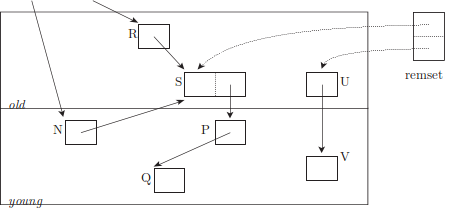
\includegraphics{figures/gen_1}
  \caption[Διαγενεαλογικοί δείκτες]
    {Διαγενεαλογικοί δείκτες. Η διατήρηση των ζωντανών αντικειμένων
     της νέας γενεάς χωρίς την εξερεύνηση όλου του σωρού, απαιτεί
     ένα μηχανισμό και μια δομή δεδομένων για την καταγραφή των
     αντικειμένων S και U που περιέχουν δείκτες προς αντικείμενα
     της νέας γενεάς.}
  \label{fig:gen_1} 
\end{figure}

Οι ρίζες μιας γενεάς πρέπει να ανακαλυφθούν πριν αυτή συλλεχθεί.
Οι ρίζες για μια γενεά δεν περιλαμβάνουν μόνο τους δείκτες που
βρίσκονται σε καταχωρητές, στη στοίβα και σε καθολικές μεταβλητές
αλλά και δείκτες προς αντικείμενα της γενεάς από αντικείμενα
που ζουν σε κάποια άλλη περιοχή του σωρού η οποία δε συλλέγεται
ταυτόχρονα με τη γενεά. Αυτές οι περιοχές τυπικά περιλαμβάνουν
τις παλαιότερες γενεές αλλά και περιοχές εκτός του γενεαλογικού
σωρού όπως χώροι που φιλοξενούν πολύ μεγάλα αντικείμενα και
χώροι που δε συλλέγονται ποτέ, όπως οι χώροι που αποθηκεύουν
αθάνατα αντικείμενα και πιθανώς κώδικα. Όπως έχουμε εξηγήσει,
οι διαγενεαλογικοί δείκτες δημιουργούνται είτε με την αρχικοποίηση
εγγραφών κατά τη δημιουργία των αντικειμένων, είτε από ενημερώσεις
πεδίων δεικτών αντικειμένων από τον τροποποιητή είτε τέλος κατά
την μετακίνηση αντικειμένων σε διαφορετικές γενεές. Γενικά, οι
δείκτες αυτοί πρέπει να εντοπίζονται τη στιγμή της δημιουργίας
τους και να καταγράφονται ώστε να μπορούν να χρησιμοποιηθούν
ως ρίζες κατά τη συλλογή μιας γενεάς. Κάθε δείκτης που πρέπει
να καταγράφεται καλείται συνήθως και \textbf{ενδιαφέρων δείκτης}.

\subsection{Σύνολα ανάμνησης}
Οι δομές δεδομένων που χρησιμοποιούνται για την καταγραφή διαγενεαλογικών
δεικτών ονομάζονται \textbf{σύνολα ανάμνησης}. Τα σύνολα ανάμνησης
καταγράφουν τη θέση προέλευσης διαφόρων δεικτών μεταξύ διαφορετικών
χώρων του σωρού. Καταγράφεται η προέλευση και όχι ο προορισμός
ενός δείκτη για δύο λόγους. Πρώτον, επιτρέπεται σε ένα μετακινούντα
συλλέκτη να ενημερώσει το πεδίο προέλευσης με τη νέα διεύθυνση
ενός αντικειμένου που έχει αντιγραφεί η προαχθεί. Δεύτερον ένα
πεδίο προέλευσης κάποιου δείκτη μπορεί να ενημερωθεί πολλές φορές
στο ανάμεσα σε δύο διαδοχικούς κύκλους συλλογής και έτσι αν ο
συλλέκτης θυμάται την προέλευση του δείκτη, εξασφαλίζεται πώς
αυτός επεξεργάζεται το πραγματικό αντικείμενο προς το οποίο
αναφέρεται ο δείκτης τη στιγμή της προέλευσης και όχι τα αντικείμενα
προορισμούς ενδιάμεσων παρωχημένων τιμών του αυτού. Επομένως το
σύνολο ανάμνησης για κάθε γενεά αποθηκεύει τις θέσεις εκείνες
στις οποίες βρίσκεται ένας πιθανόν ενδιαφέρων δείκτης προς κάποιο
αντικείμενο της γενεάς. Οι διάφορες υλοποιήσεις των συνόλων ανάμνησης 
διαφέρουν ως προς την ακρίβεια με την οποία καταγράφουν τέτοιες
θέσεις. Η επιλογή της ακρίβειας προσπαθεί να επιτύχει ένα
συμβιβασμό μεταξύ της επιβάρυνσης του τροποποιητή, του απαιτούμενου
χώρου αποθήκευσης των συνόλων ανάμνησης και το κόστος επεξεργασίας
τους από το συλλέκτη.

Εμφανώς είναι επιθυμητός ο εντοπισμός και η καταγραφή όσο το
δυνατόν λιγότερων δεικτών. Οι ενημερώσεις δεικτών από
το συλλέκτη κατά τη μετακίνηση αντικειμένων εντοπίζονται εύκολα.
Οι εγγραφές δεικτών από τον τροποποιητή μπορούν να ανιχνευθούν
από ένα φράγμα εγγραφής λογισμικού, το οποίο μπορεί να εισαχθεί
αυτόματα από το μεταγλωττιστή πριν από κάθε λειτουργία εγγραφής
ενός δείκτη. Αυτό βέβαια δεν είναι εφικτό αν ο μεταγλωττιστής
της γλώσσας είναι μη συνεργατικός. Στην περίπτωση αυτή, οι
θέσεις των λειτουργιών εγγραφής μπορούν συχνά να καθορισθούν
από το διαχειριστή εικονικής μνήμης του λειτουργικού συστήματος.

Η συχνότητα των ενημερώσεων δεικτών διαφέρει μεταξύ των
διαφορετικών γλωσσών προγραμματισμού και των υλοποιήσεων αυτών.
Ο Zorn εφαρμόζοντας στατική ανάλυση σε μια σουίτα προγραμμάτων
σε Lisp \cite{DBLP:conf/lfp/Zorn90}, υπολόγισε τη συχνότητα
των ενημερώσεων δεικτών από 13\% έως και 15\%, ενώ ο Appel
υπολόγισε μία χαμηλότερη στατική συχνότητα της τάξης του 3\% 
στη γλώσσα Lisp \cite{DBLP:journals/ipl/Appel87}, και μία
δυναμική συχνότητα χρόνου εκτέλεσης της τάξης του 1\% για
τη γλώσσα ML \cite{DBLP:journals/spe/Appel89a}. Οι Dieckmann
και H{\"o}lzle \cite{DBLP:conf/ecoop/DieckmannH99} βρήκαν
τέλος πώς τα προγράμματα σε γλώσσα Java μπορεί να διαφέρουν
σημαντικά ως προς τη συχνότητα των ενημερώσεων δεικτών
(το ποσοστό των προσβάσεων στο σωρό που αφορούσε αποθηκεύσεις
τιμών σε πεδία δείκτες κυμαινόταν από 6\% έως και 70\%).

Αν τα πλαίσια αυτά σαρώνονται ως μέρος του συνόλου ριζών σε
κάθε συλλογή, είναι δυνατή η ανακάλυψη των θέσεων τους που
περιέχουν δείκτες. Επιπλέον, αν ο μεταγλωττιστής μπορεί να
ταυτοποιήσει τις λειτουργίες εγγραφής στη στοίβα, τότε δε
χρειάζεται να τοποθετήσει φράγματα εγγραφής πριν από αυτές.
Επιπρόσθετα, πολλοί δείκτες αναφέρονται σε αντικείμενα της
ίδιας διαμέρισης. Παρότι οι αποθηκεύσεις πιθανώς εντοπίζονται,
οι δείκτες δεν είναι ενδιαφέροντες από γενεαλογική άποψη και
δε χρειάζεται να καταγραφούν.

Εάν επιβληθεί μια τάξη ως προς τη σειρά συλλογής των διαφόρων
γενεών, το πλήθος των διαγενεαλογικών δεικτών που πρέπει να
καταγραφούν μπορεί να μειωθεί ακόμη περισσότερο. Εξασφαλίζοντας
πώς οποτεδήποτε συλλέγεται μια γενεά συλλέγονται και όλες οι
νεότερες γενεές από αυτή, μόνο οι δείκτες από παλαιά αντικείμενα
προς νέα αντικείμενα πρέπει να καταγραφούν. Πολλές λειτουργίες
εγγραφής δεικτών αφορούν την αρχικοποίηση πεδίων αντικειμένων
που μόλις έχουν δημιουργηθεί. Εξ 'ορισμού, οι δείκτες αυτοί
αναφέρονται σε γηραιότερα αντικείμενα. Δυστυχώς πολλές γλώσσες
διαχωρίζουν την εκχώρηση μνήμης για ένα αντικείμενο από την
αρχικοποίηση των πεδίων του τελευταίου, καθιστώντας δύσκολη τη
διάκριση των λειτουργιών εγγραφής δεικτών που δεν αφορούν
αρχικοποιήσεις και πιθανόν δημιουργούν δείκτες από μια παλαιά
γενεά προς μία νέα γενεά. Άλλες γλώσσες παρέχουν περισσότερη
υποστήριξη στο μεταγλωττιστή όσον αφορά την αναγνώριση των
λειτουργιών εγγραφής δεικτών που δε χρειάζονται κάποιο φράγμα
εγγραφής. Η πλειοψηφία των λειτουργιών εγγραφής δεικτών σε μία
αγνή οκνηρή γλώσσα συναρτησιακού προγραμματισμού όπως η Haskell
κάνει τους δείκτες να αναφέρονται σε γηραιότερα αντικείμενα.
Η γλώσσα ML απαιτεί από τον προγραμματιστή να σημειώσει ρητά
τις τροποποποιήσιμες μεταβλητές: οι λειτουργίες εγγραφής αυτών
των μεταβλητών είναι η μόνη πηγή δημιουργίας δεικτών από
αντικείμενα μιας παλαιάς γενεάς προς αντικείμενα μιας νέας
γενεάς. Το σκηνικό στις αντικειμενοστρεφείς γλώσσες προγραμματισμού
από την άλλη όπως για παράδειγμα στη Java είναι πιο πολύπλοκο.
Η φιλοσοφία προγραμματισμού εδώ βασίζεται στην ενημέρωση της
κατάστασης αντικειμένων, κάτι που οδηγεί φυσικά στη δημιουργία
περισσότερων δεικτών από αντικείμενα μιας νέας γενεάς προς
αντικείμενα μιας παλαιάς γενεάς.

Σε σωρούς με πολλαπλές ανεξάρτητα συλλεγόμενες γενεές απαιτείται
διαφορετική τεχνική φιλτραρίσματος δεικτών. Για παράδειγμα ένας
συλλέκτης μπορεί να εφαρμόσει ευριστικές για να αποφασίσει
ποιο χώρο θα συλλέξει, δίνοντας προτεραιότητα στους χώρους
με το μικρότερο πλήθος ζωντανών αντικειμένων. Στην περίπτωση
αυτή το φράγμα εγγραφής πρέπει να καταγράψει δείκτες και προς
τις δύο κατευθύνσεις. Καθώς αυτή η σχεδίαση αναμένεται να αυξήσει
το πλήθος των διαγενεαλογικών δεικτών προς καταγραφή, είναι
βέλτιστη για χρήση σε μια υλοποίηση όπου το μέγεθος του συνόλου
ανάμνησης είναι ανεξάρτητο του πλήθους των ενθυμούμενων
δεικτών.

\section{Διαχείριση χώρου}
Η νεότερη γενεά συνήθως διαχειρίζεται με αντιγραφή. Τα επιζώντα
αντικείμενα αντιγράφονται είτε σε ένα φρέσκο ημιχώρο στην
ίδια γενεά είτε σε μία παλαιότερη γενεά. Οι συλλογές των
νέων γενεών αναμένεται να είναι συχνές και σύντομες σε διάρκεια,
λαμβάνοντας υπόψη την ασθενή γενεαλογική υπόθεση. Από την άλλη
πλευρά, οι συλλογές των παλαιότερων γενεών αναμένεται να είναι
λιγότερες συχνές αλλά να διαρκούν πολύ, καθώς πρέπει μαζί με
αυτές πρέπει να συλλεγούν και οι νεότερες γενεές προκειμένου
να αποφευχθεί το κόστος χρήσης ενός φράγματος εγγραφής που
καταγράφει δείκτες και προς τις δύο κατευθύνσεις. Συνήθως
μια συλλογή της παλαιότερης γενεάς θα συλλέξει όλες τις περιοχές
του σωρού εκτός ίσως από την περιοχή όπου φιλοξενούνται αθάνατα
αντικείμενα (παρότι οι δείκτες της περιοχής αυτής αντιμετωπίζονται
ως ρίζες και ενδέχεται να ενημερωθούν). Μια πλήρης συλλογή του
σωρού δεν απαιτεί τη χρήση συνόλων ανάμνησης, εκτός ίσως για
τοποθεσίες της περιοχής αθάνατων αντικειμένων στην περίπτωση
που αυτή δε σαρώνεται.

Έχει προταθεί μία ευρεία γκάμα στρατηγικών διαχείρισης της
παλαιότερης γενεάς. Η συλλογή με αντιγραφή μεταξύ ημιχώρων
δεν είναι η καλύτερη επιλογή ειδικά αν λάβει κανείς υπόψη
πώς και η νεότερη γενεά συλλέγεται με την ίδια τεχνική: η
απαίτηση της συλλογής για την διατήρηση ενός εφεδρικού χώρου
αντιγραφής καταλήγει να δαπανά το μισό χώρο στο σωρό, κάτι
που έχει ως αποτέλεσμα την αύξηση της συχνότητας των συλλογών
όλων των γενεών. Επίσης τα μακρόβια αντικείμενα μετακινούνται
συνέχεια. Ο Blackburn κ.ά ισχυρίζονται \cite{DBLP:conf/icse/BlackburnCM04}
πώς η συλλογή με σήμανση και εκκαθάριση προσφέρει καλύτερη
χρησιμοποίηση του διαθέσιμου χώρου, ειδικά σε μικρούς σωρούς.
Το μειονέκτημα της συλλογής με σήμανση και εκκαθάριση, η οποία
δεν μετακινεί τα ζωντανά αντικείμενα, αφορά στη μείωση της
επίδοσης από την πιθανό κατακερματισμό. Η λύση είναι η προσθήκη
μιας φάσης συμπύκνωσης της παλαιάς γενεάς οποτεδήποτε ο
κατακερματισμός επηρεάζει δυσμενώς την επίδοση. Η συμπύκνωση
επίσης μπορεί να διαχειρισθεί τα μακρόβια αντικείμενα με
ειδικό τρόπο, όπως είδαμε στο κεφάλαιο~\ref{ch:mrkcmp}.

Οι γενεαλογικοί συλλέκτες σχεδόν πάντοτε διαχωρίζουν τις
γενεές τους φυσικά και όχι εικονικά. Αυτό απαιτεί τη διαχείριση
των νεότερων γενεών από συλλογή με αντιγραφή. Ένας προσαρμοστικός
συλλέκτης αντιγραφής σαν και αυτόν του Appel για παράδειγμα
συντηρητικά απαιτεί ο εφεδρικός χώρος αντιγραφής να έχει το
ίδιο μέγεθος με την περιοχή που συλλέγεται καθώς στην χειρότερη
περίπτωση όλα τα αντικείμενα μπορεί να επιβιώσουν. Στην πράξη
βέβαια τα περισσότερα αντικείμενα δεν επιβιώνουν από μια συλλογή
της νέας γενεάς.

Ο McGachey κ.ά. \cite{DBLP:conf/iwmm/McGacheyH06} ισχυρίζονται
πώς η χρησιμοποίηση του χώρου μπορεί να βελτιωθεί με τη διατήρηση
ενός μικρότερου μεγέθους εφεδρικού χώρου αντιγραφής και την
εναλλαγή μεταξύ συλλογής με αντιγραφή σε συλλογή με σήμανση και
συμπύκνωση οποτεδήποτε το μέγεθος του χώρου αυτού γίνει πολύ
μικρό. 

\section{Ανακεφαλαίωση και θέματα προς εξέταση}
Η γενεαλογική συλλογή σκουπιδιών έχει αποδειχθεί αποδοτική,
προσφέροντας σημαντικές βελτιώσεις επίδοσης για μια ευρεία
γκάμα εφαρμογών. Μειώνοντας το μέγεθος της νεότερης γενεάς
και επικεντρώνοντας τις προσπάθειες συλλογής σε αυτήν, οι
αναμενόμενοι χρόνοι παύσης μπορούν να ελαττωθούν σε τέτοιο
σημείο ώστε να περνούν σχεδόν απαρατήρητοι σε διάφορα περιβάλλοντα.
Η τεχνική της γενεαλογικής συλλογής σκουπιδιών μπορεί επίσης
να αυξήσει τη γενική ρυθμαπόδοση του συλλέκτη με δύο τρόπους.
Πρώτον, μειώνει τη συχνότητα επεξεργασίας των μακρόβιων αντικειμένων
και επομένως όχι μόνο μειώνει την υπολογιστική προσπάθεια αλλά
επιπλέον δίνει στα αντικείμενα αυτά περισσότερο χρόνο για να
πεθάνουν (και έτσι να μην χρειαστεί να εξιχνιαστούν οι υπογράφοι
των οποίων είναι ρίζες). Δεύτερον, οι γενεαλογικοί συλλέκτες
συνήθως εκχωρούν μνήμη για την αποθήκευση νέων αντικειμένων
σειριακά σε μία περιοχή βρεφοκομείου. Η σειριακή εκχώρηση έχει
ως αποτέλεσμα τη βελτίωση του ρυθμού αστοχιών κρυφής μνήμης
καθώς το μοτίβο πρόσβασης στη μνήμη είναι προβλέψιμο και
επιπλέον οι περισσότερες εγγραφές αφορούν τα νεότερα αντικείμενα.

Η γενεαλογική συλλογή σκουπιδιών ωστόσο δεν είναι πανάκεια.
Η αποδοτικότητά της εξαρτάται άμεσα από την κατανομή της διάρκειας
των αντικειμένων μιας εφαρμογής. Αν η μεγάλη πλειοψηφία των
αντικειμένων δεν πεθαίνει νέα, η γενεαλογική συλλογή σκουπιδιών
δεν είναι κατάλληλη.

Επιπλέον, η γενεαλογική συλλογή σκουπιδιών βελτιώνει μόνο
τους αναμενόμενους χρόνους παύσης. Τελικώς, ο συλλέκτης πρέπει
να συλλέξει όλο το σωρό και συνεπώς η γενεαλογική συλλογή από
μόνη της δεν μπορεί να επιλύσει το πρόβλημα της μείωσης του
χρόνου παύσης \textbf{χειρότερης περίπτωσης}, ο οποίος αυξάνεται
υπερβολικά πολύ σε μεγάλους σωρούς. Συνεπώς, η γενεαλογική
συλλογή σκουπιδιών δεν μπορεί να παράσχει τις απαιτούμενες εγγυήσεις
ενός σκληρού συστήματος πραγματικού χρόνου όπου οι προθεσμίες
πρέπει πάντοτε να τηρούνται.

Η υλοποίηση της συλλογής σκουπιδιών είναι απλούστερη αν υπάρχει
η δυνατότητα μετακίνησης αντικειμένων προς διάκριση των παλαιών
αντικειμένων από τα νέα. Ο φυσικός διαχωρισμός δεν προσφέρει
μόνο το πλεονέκτημα της τοπικότητας που συζητήθηκε παραπάνω,
αλλά επίσης πιο αποδοτικούς ελέγχους χώρου, οι οποίοι είναι
απαραίτητοι στο φράγμα εγγραφής αλλά και κατά την εξιχνίαση
της νεότερης γενεάς. Τα αντικείμενα πάντως μπορούν να διαχωρίζονται
με βάση την ηλικία τους και εικονικά, χρησιμοποιώντας πιθανώς
ένα bit στην επικεφαλίδα τους ή σε κάποιο bitmap.

Οι γενεαλογικοί συλλέκτες εγείρουν μια πληθώρα διαφορετικών
ερωτημάτων όσον αφορά τόσο τις επιλογές υλοποίησης όσο και
τις απαιτήσεις του τελικού χρήστη μιας εφαρμογής. Η υλοποίηση
γενεαλογικών συλλεκτών περιλαμβάνει πολύ περισσότερες σχεδιαστικές
επιλογές από την επιλογή του μεγέθους του σωρού.

Η πρώτη απόφαση υλοποίησης συνήθως αφορά το αν ο σωρός θα
οργανωθεί σε δύο ή περισσότερες γενεές. Η απάντηση εξαρτάται
πρωτίστως από τις κατανομές της διάρκειας ζωής των εφαρμογών
για τις οποίες ο συλλέκτης θα παρέχει υποστήριξη. Εάν ένα
σημαντικό ποσοστό των αντικειμένων αναμένεται να επιβιώσουν
από τη νεότερη γενεά αλλά να πεθάνουν σύντομα μετά την προαγωγή
τους, τότε ίσως αξίζει η προσθήκη ενδιάμεσων γενεών. Τα περισσότερα
συστήματα αυτόματης διαχείρισης μνήμης με γενεαλογική συλλογή
σκουπιδιών ωστόσο από προεπιλογή περιλαμβάνουν δύο γενεές και
μια αθάνατη γενεά. Η χρήση πολλαπλών γενεών προσπαθεί να λύσει
το πρόβλημα της πρόωρης προαγωγής αντικειμένων. Υπάρχουν και
άλλοι τρόποι επίλυσής του.

Αρχικά, ο ρυθμός προαγωγής εξαρτάται από το μέγεθος της νέας
γενεάς: μια μεγαλύτερη νέα γενεά προσφέρει περισσότερο χρόνο
σε ένα αντικείμενο για να πεθάνει. Μερικοί γενεαλογικοί συλλέκτες
επιτρέπουν στο χρήστη να ρυθμίσει ένα σταθερό μέγεθος για τη
νεότερη γενεά. Άλλοι πάλι επιτρέπουν στη νεότερη γενεά να
αυξάνεται δυναμικά μέχρις ότου καταλάβει όλο το σωρό (εκτός
από ήδη δεσμευμένες περιοχές, όπως η παλαιά γενεά και πιθανόν
μια εφεδρική περιοχή αντιγραφής). Οι πιο εξεζητημένοι συλλέκτες
σκουπιδιών πάντως μπορούν να μεταβάλλουν το μέγεθος της νεότερης
γενεάς προς ικανοποίηση συγκεκριμένων προδιαγραφών σχετικά
με τους χρόνους παύσης, λαμβάνοντας αποφάσεις για την αλλαγή
του μεγέθους με βάση την παρακολούθηση του προφίλ της συμπεριφοράς
του συλλέκτη.

Δεύτερον, η προαγωγή μπορεί να περιορισθεί ελέγχοντας την ηλικία
κατά την οποία τα αντικείμενα προάγονται. Η τεχνική της μαζικής
προαγωγής μεταφέρει όλους τους επιζώντες μιας συλλογής της νεότερης
γενεάς σε μια παλαιότερη γενεά. Αυτή η πολιτική προαγωγής έχει
μάλιστα την απλούστερη υλοποίηση, καθώς τα ενθυμούμενα σύνολα
για τη νεότερη γενεά μπορούν να παραμερισθούν μετά το πέρας
της συλλογής. Εναλλακτικά, ένας συλλέκτης μπορεί να απαιτεί
από ένα αντικείμενο να επιβιώσει περισσότερους του ενός κύκλων
συλλογής πριν το προάγει. Στην περίπτωση αυτή, είναι απαραίτητος
ένας μηχανισμός καταγραφής της ηλικίας των αντικειμένων. Αυτό
μπορεί να επιτευχθεί είτε με τη χρήση κάποιων bits από την
επικεφαλίδα των αντικειμένων, με τη διαίρεση μιας γενεάς σε
σε υποχώρους ο καθένας από τους οποίους φιλοξενεί αντικείμενα
διαφορετικής ηλικίας, είτε με συνδυασμό των δύο. Οι συνηθισμένες
διαμορφώσεις περιλαμβάνουν σχήματα οργανωμένα σε βήματα και
σχήματα που περιλαμβάνουν μια περιοχή εδέμ και ημιχώρους επιζώντων.

Τέλος, είναι πολλές φορές πιθανή η αποφυγή της υποχρέωσης
προαγωγής ορισμένων αντικειμένων. Πολλοί συλλέκτες σκουπιδιών
δεσμεύουν μια αθάνατη περιοχή για αντικείμενα που θα επιβιώσουν
μέχρι το τέλος του προγράμματος. Τα αντικείμενα αυτά συχνά μπορούν
να αναγνωρισθούν είτε κατά την υλοποίηση του συλλέκτη είτε από
το μεταγλωττιστή. Τέτοια αντικείμενα συνήθως περιλαμβάνουν
τις δομές δεδομένων του συλλέκτη καθώς αντικείμενα που αναπαριστούν
τον υπό εκτέλεση κώδικα.

Οι ρυθμοί προαγωγής μπορούν επίσης να επηρεάσουν το κόστος του
φράγματος εγγραφής καθώς επίσης και το μέγεθος των ενθυμούμενων
συνόλων. Υψηλότεροι ρυθμοί προαγωγής προκαλούν τη δημιουργία
περισσότερων διαγενεαλογικών δεικτών που πρέπει να καταγραφούν.
Εάν αυτό επηρεάζει ή όχι την απόδοση των φραγμάτων εγγραφής
εξαρτάται από την υλοποίηση.

Η συχνότητα κλήσης των φραγμάτων εγγραφής εξαρτάται επίσης
από το αν οι διαφορετικές γενεές μπορούν να συλλεχθούν ανεξάρτητα.
Η ανεξάρτητη συλλογή των γενεών απαιτεί την καταγραφή όλων
των διαγενεαλογικών δεικτών. Η εγκατάλειψη αυτής της ευελιξίας
σημαίνει πώς την ταυτόχρονη συλλογή όλων των νεότερων γενεών
οποτεδήποτε συλλέγεται η παλαιότερη γενεά και επιτρέπει την
καταγραφή μόνο των δεικτών με προέλευση κάποια παλαιότερη
γενεά και προορισμό κάποια νεότερη γενεά (οι οποίοι αναμένεται
να είναι σημαντικά λιγότεροι σε πλήθος). Σημειώνοντας το
αντικείμενο και όχι το συγκεκριμένο πεδίο αυτού ως πιθανή
προέλευση ενός διαγενεαλογικού δείκτη, το κόστος σε χώρο για
την αποθήκευση των συνόλων ανάμνησης μπορεί να μειωθεί.

Οι διαφορετικοί μηχανισμοί που χρησιμοποιεί ο τροποποιητής για
την καταγραφή των πιθανών προελεύσεων διαγενεαλογικών δεικτών
επηρεάζουν το κόστος της συλλογής. Παρότι μηχανισμοί λιγότερο
ακριβείς μπορεί να μειώσουν το κόστος του φράγματος εγγραφής,
αυτοί μπορεί να αυξήσουν το φορτίο εργασίας του συλλέκτη.
Η καταγραφή του πεδίου προέλευσης με χρήση σειριακών απομονωτών
αποθήκευσης είναι ο πιο ακριβής μηχανισμός παρότι ένας απομονωτής
ενδέχεται να περιλαμβάνει κάποιες καταχωρίσεις εις διπλούν.
Η καταγραφή του αντικειμένου προέλευσης από την άλλη πλευρά
απαιτεί τη σάρωση του αντικειμένου για την εύρεση διαγενεαλογικών
δεικτών.

\end{greek}



